% Template for ICASSP-2026 paper; to be used with:
%          spconf.sty  - ICASSP/ICIP LaTeX style file, and
%          IEEEbib.bst - IEEE bibliography style file.
% --------------------------------------------------------------------------
\documentclass{article}
\usepackage{spconf,amsmath,graphicx,hyperref, amssymb}
\usepackage{siunitx}
% Example definitions.
% --------------------
\def\x{{\mathbf x}}
\def\L{{\cal L}}

% Title.
% ------
\title{X-Ray Near-Field Holotomography Reconstruction Using Implicit Neural Representations}
%
% Single address.
% ---------------
%\name{Author(s) Name(s)\thanks{Thanks to XYZ agency for funding.}}
%\address{Author Affiliation(s)}
%
% For example:
% ------------
%\address{School\
%\vfill\pagebreak
%	Department\\
%	Address}
%
% Two addresses (uncomment and modify for two-address case).
% ----------------------------------------------------------
%	\name{a,b,c}{d,e,f}
\name{
	Johannes Gruen$^{1}$\thanks{We acknowledge DESY (Hamburg, Germany), a member of the Helmholtz Association HGF, for the provision of experimental facilities, and DASHH, Data Science in Hamburg - Helmholtz Graduate School  for the Structure of Matter, for financial support. Parts of this research were carried out at the PETRA III beamline P05: Beamtime-ID (11019330).
	This research was supported in part through the Maxwell computational resources operated at DESY. This research was supported by Hi-Acts, an innovation platform under the grant of the Helmholtz Association HGF. We acknowledge J. Dora for his help tuning ASRM parameters.}, 
	Sebastian Eberle$^{1}$, 
	Imke Greving$^{2}$,
Silja Flenner$^{2}$,}{
	Martin Burger$^{3,4}$, 
	Christian G. Schroer$^{1,3,5}$,
	Johannes Hagemann$^{1}$
}

\address{
	$^{1}$Center for X-Ray and Nano Science CXNS, Deutsches Elektronen Synchroton DESY, \\
	$^{2}$ Institute of Materials Physics, Helmholtz-Zentrum Hereon\\
	$^{3}$Helmholtz Imaging, Deutsches Elektronen Synchroton DESY\\ 
	$^{4}$Department Mathematik, Universität Hamburg\\ 
	$^{5}$Department Physik, Universität Hamburg
}
\begin{document}
\ninept
\frenchspacing
%
\maketitle
%
\begin{abstract}
	X-ray near-field holotomography provides non-destructive, in situ 3D visualization of specimen interiors at nanometer-scale resolution.
Reconstruction traditionally involves two separate steps: first retrieving the projected phase for different rotation angles, then applying tomographic reconstruction to obtain a 3D volume from 2D projections.
Both steps are ill-posed inverse problems and separating them leads to information loss, due to reconstruction errors.
Recent advances in implicit neural representations (INRs) have demonstrated remarkable capabilities in scene rendering and tomographic reconstruction.
In this work, we propose a unified INR-based framework that jointly solves the phase retrieval and tomographic reconstruction problems.
This joint formulation enforces 3D consistency, resulting in significantly improved phase, absorption, and volumetric reconstructions.
Moreover, INRs provide substantial data compression.
This compression reduces storage requirements by $95\%$, which is particularly important with the advent of fourth-generation synchrotron sources and the corresponding growth in data volume.
\end{abstract}
%
\begin{keywords}
X-ray near-field holotomography, Implicit neural representations
\end{keywords}
%
\section{Introduction}
\label{sec:intro}
X-ray computed tomography (CT) is a widely employed technique for reconstructing three-dimensional (3D) volumes from two-dimensional (2D) projection data.
Conventional CT relies on absorption contrast, which only works on sufficiently large features. 
In the nanometer regime, however, phase contrast becomes dominant, motivating the development of X-ray near-field holography, which can be modeled using the Fresnel propagation.
This approach to microscopy is particularly advantageous for characterization of sub-$\mu$m structures, such as biological~\cite{vesely3DXrayNanotomography2021a,flennerHardXrayNanoholotomography2020b,gerhardtThreedimensionalArchitectureLinearized2025} and material science specimen~\cite{reimersDevelopmentBioreactorCoupledFlowCell2023}.

In this setting, the conventional tomographic reconstruction problem is augmented by an additional phase retrieval problem, which must be solved for each projection image.
Phase retrieval is inherently nonlinear and ill-posed, as it seeks to reconstruct the complex-valued refractive index from real-valued intensity measurements.
Furthermore, the contrast transfer function (CTF) of the Fresnel propagator exhibits multiple zeros, corresponding to spatial frequencies with no measurable phase information, which further exacerbates the ill-posedness of the inverse problem.

A common strategy to mitigate this limitation is to record projections at multiple propagation distances, as introduced by Misell~\cite{Misell_1973},
and demonstrated for hard X rays by Cloetens \textit{et~al.}~\cite{cloetensHolotomographyQuantitativePhase1999a}.
More recently, several studies have shown that it is possible to reconstruct the complex refractive index from a measurement acquired at a single propagation distance.
This is achieved by incorporating prior knowledge, such as physically motivated constraints or other regularizations, which can yield accurate and stable reconstructions~\cite{doraArtifactsuppressingReconstructionStrongly2024,fienupReconstructionSupportObject1982,wittwerPhaseRetrievalFramework2022}.

An alternative approach to introducing priors is to enforce three-dimensional consistency, also known as Helgason-Ludwig consistency, by jointly solving the tomographic reconstruction and phase retrieval problems~\cite{ludwigRadonTransformEuclidean1966,helgasonRadonTransformEuclidean1965}.
This coupling imposes a strong constraint on the recovered phase maps, effectively constraining them to be consistent with the underlying 3D structure.
For non-rotational symmetric objects joint reconstruction also reduces the loss of information due to zeros in the CTF, as the frequency changes depending on the viewing angle, allowing the 3D reconstruction for a subset of angles, similar to sparse angle tomography.

The concept of joint 3D reconstruction is not new.
As early as 2013,  it was proposed to couple phase retrieval and tomographic reconstruction by alternating over both optimization problems~\cite{kostenkoTotalVariationMinimization2013,ruhlandtThreedimensionalPhaseRetrieval2014}.
Ruhland \textit{et~al.} could show that this approach improves the reconstruction of low-frequencies~\cite{ruhlandtThreedimensionalPhaseRetrieval2014}.
Later they proposed another approach under the assumption of optically weak objects, for which the exponential attenuation model can be linearized, leading to much faster computation compared to earlier works~\cite{ruhlandtThreedimensionalPropagationNearfield2016a}.
Linearization is not valid at the nanometer-scale, due to strong phase-shift, hence, the method is not applicable in our case.
The principal limitation of the earlier methods, however, lies in their computational and memory requirements, as the reconstruction volume scales cubically with resolution, making it quickly prohibitive.

\begin{figure*}
	\centering
	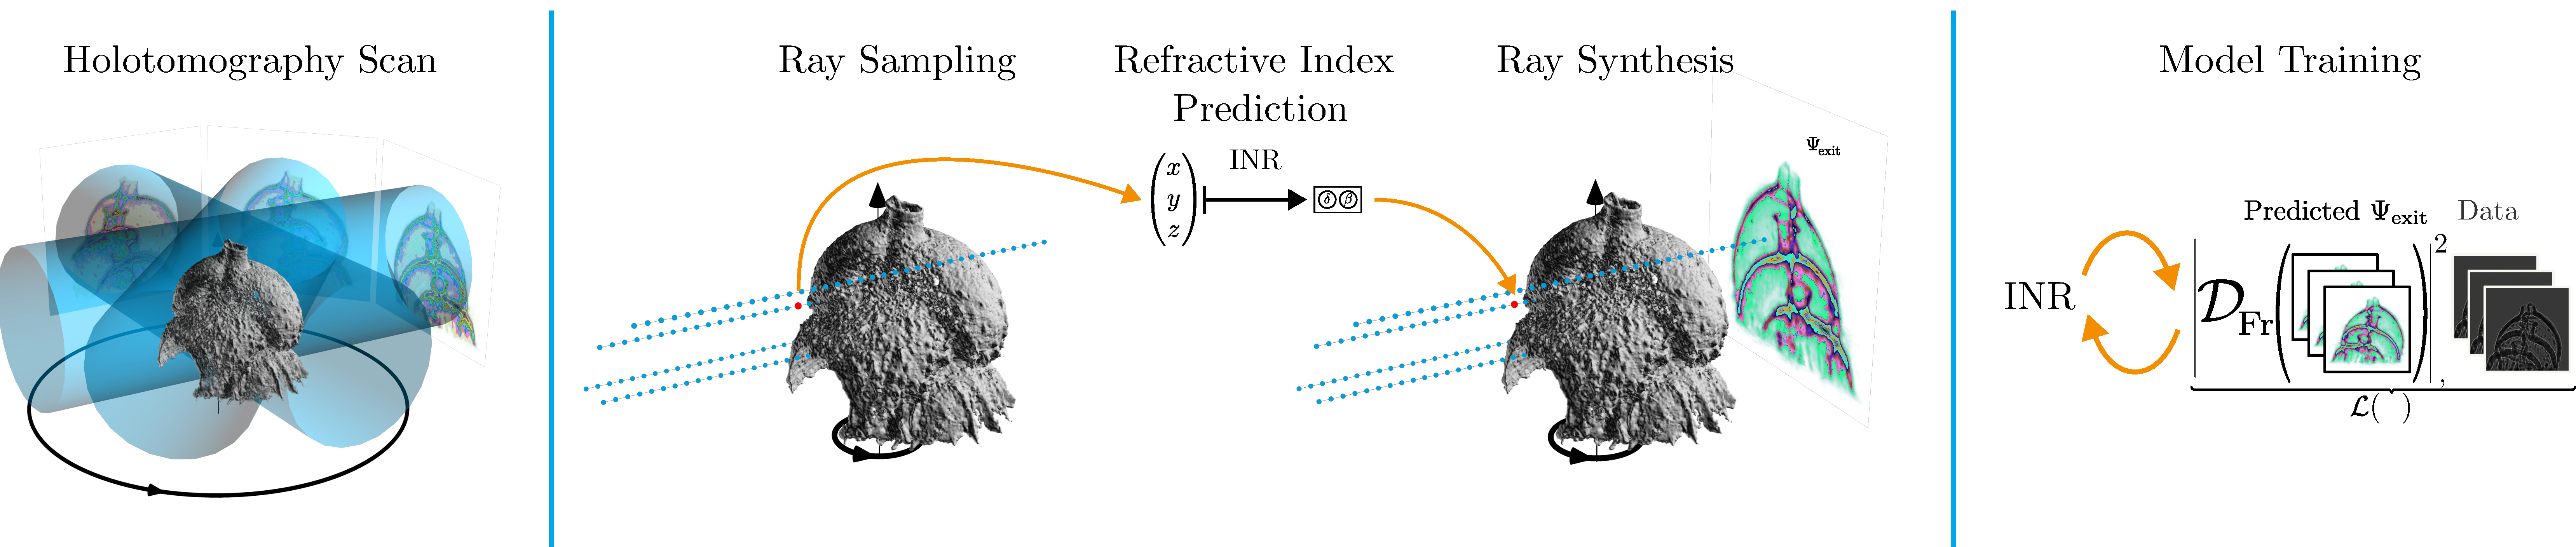
\includegraphics[width=1\linewidth]{images/overview.pdf}
	\caption{Left: Measurement process.
		Object is rotated while measuring, leading to angular dependent holograms.
		Center: Description of the ray sampling.
		For a given position the INR predicts phase and absorption, which is then integrated along the ray.
		Right: Training process.
		The resulting 2D image is then propagated to the detector and the model is trained by minimizing the loss.
	}
	\label{fig:overiew}
\end{figure*}


A promising alternative is to represent the volume in a continuous, implicit form rather than on a discrete voxel grid~\cite{mildenhallNeRFRepresentingScenes2020a}.
In this framework, a neural network encodes the volume and can be queried at arbitrary spatial coordinates to predict the corresponding refractive index.
Such INRs are highly parameter-efficient and reduce the memory scaling issues associated with grid-based methods.
Early implementations, however, struggled to capture fine structural details, as neural networks tend to favor low-frequency components, commonly known as spectral bias~\cite{rahamanSpectralBiasNeural2019}.
Recent advances in computer vision have addressed this issue through novel network architectures and encoding schemes that enhance the representation of high-frequency information~\cite{mildenhallNeRFRepresentingScenes2020a,mullerInstantNeuralGraphics2022}.
For CT reconstruction INR-based approaches lead to state-of-the-art results~\cite{essakineWhereWeStand2025,zhaNAFNeuralAttenuation2022a}.


In this work, we present the first joint X-ray near-field holotomography reconstruction using an INR, which directly learns a continuous complex refractive index volume from holograms.

\section{Method}
\begin{figure*}
	\centering
	\includegraphics[width=\textwidth]{images/projections.pdf}
	\caption{
		Comparison of 2D phase (top row) and absorption (bottom row) reconstructions.
		The INR-based phase reconstructions are largely consistent regardless of the number of holograms used.
		Compared to ASRM, the proposed INR approach reduces fringing artifacts and yields a more uniform surface, which is not properly reconstructed using ASRM.
		Furthermore, the INR method produces promising absorption reconstructions, although the results become less stable when only 40 measurements are available.
	}
	\label{fig:projections}
\end{figure*}

\subsection{Forward Model}
The interaction of X-rays with matter results in phase shifts and absorption, characterized by the complex refractive index of the material.
Therefore, the objective is to reconstruct the refractive index of the object  
\begin{align}
	O \left( x,y,z \right) = \delta \left( x,y,z \right) + \mathrm{i} \beta \left( x,y,z \right),
	\label{eq:refractive-index}
\end{align}
where $\delta \in \mathbb{R}_{\leq 0}$ denotes the phase shift and $\beta \in \mathbb{R}_{\geq 0}$ the absorption property at position $\left( x,y,z \right) \in \mathbb{R}^{3}$.  
The reconstruction is based on a set of measured intensities $\mathcal{I}_\varphi \left( x,y \right) \in \mathbb{R}_{\geq 0}$, where $\varphi \in \left[ 0, \pi \right)$ denotes the rotation angle of the object around the $y$-axis.  
The refractive index is linked to the measured intensity via the following forward model:

The interaction of the incoming wavefield with the object is modeled as
\begin{align}
	\Psi_{ \varphi} \left( O \right) \left( x,y \right) =
	\exp \left( - \mathrm{i}k  \int_{\ell_{\varphi, x, y}} O \left( \x \right) \mathrm{d}\x \right),
\end{align}
where $\ell_{\varphi, x, y}$ denotes the line corresponding to a ray passing through the point $\left( x,y \right)$ at angle $\varphi$, and $k=\frac{2\pi}{\lambda}$ denotes the wavenumber, where $\lambda$ is the wavelength.
This is commonly referred to as the thin-object approximation~\cite{paganinCoherentXrayOptics2006a}.  
Within this work, it is assumed that the incoming wavefield is accounted for by applying a flat-field correction~\cite{doraArtifactsuppressingReconstructionStrongly2024}.

Propagation of the wavefield through free space is described by the Fresnel approximation:  
\begin{align}
	\mathcal{D}_{\text{Fr}} \left( \Psi_{ \varphi} \right) = 
	\mathcal{F}^{-1} \left[ 
		\exp \left( - \mathrm{i} \pi \frac{k_{x}^{2} + k_{y}^{2}}{\text{Fr}} \right) 
		\cdot \mathcal{F} \left( \Psi_{ \varphi} \right)
	\right],
	\label{eq:fresnel}
\end{align}
where $\mathcal{F}$ and $\mathcal{F}^{-1}$ denote the Fourier transform and its inverse, and the Fresnel number $\text{Fr}$ characterizes the geometry of the experimental setup \cite{paganinCoherentXrayOptics2006a}.
While Fresnel propagation yields a complex-valued field, the detector can only record the corresponding intensities
\begin{align}
	\mathcal{I} = \left| \mathcal{D}_{\text{Fr}} \left( \Psi_{ \varphi} \right) \right|^{2},
\end{align}
i.e. the measurement loses the direct phase and absorption information yielding an ill-posed inverse problem.


\subsection{Implicit Neural Representation}
As shown in Figure~\ref{fig:overiew}, the goal of the reconstruction is to recover the object by evaluating the refractive index along multiple sampling points of each ray, effectively approximating the line integral through the volume. 
For each rotation angle, this is performed across all $\left( x,y \right)$ detector coordinates to generate a 2D projection, which is then Fresnel-propagated and compared to the measured hologram intensities.
Using a gradient step, the reconstructed volume is updated until it converges.

In principle, a simple voxel grid could be employed, where all points are sampled explicitly.  
However, this approach results in a number of free variables scaling cubical with the size of the detector.  
In our case, this would correspond to approximately 16~billion model parameters, leading to severe computational and memory limitations.  

On the other hand, in most cases volumetric samples typically consist of approximately uniform regions separated by sharp boundaries.  
Hence, neighboring voxels are strongly correlated, allowing a significant reduction in the number of parameters by exploiting this spatial redundancy.  
One way to achieve this is through a multilayer perceptron (MLP), which can theoretically approximate any continuous function.  
In practice, however, MLPs tend to favor low-frequency components, limiting their ability to represent fine details.  
This limitation has been mitigated by encoding schemes such as \emph{frequency encoding} and \emph{hash encoding}~\cite{mullerInstantNeuralGraphics2022,mildenhallNeRFRepresentingScenes2020a}.  
In this work, we adopt hash encoding, as it yields smoother reconstructions compared to frequency encoding.  

Practically, hash encoding is implemented as follows:  
the volume is represented across $L$ resolution levels, i.e., $L$ voxel grids with increasing resolution.  
For a given level $l$ a coordinate $\mathbf{x} \in \mathbb{R}^{3}$ is scaled by the level's resolution, each surrounding grid point $\tilde{\mathbf{x}} \in \mathbb{Z}^{3}$ is mapped to a hash table entry as follows:
If the number of vertices at resolution $l$ is smaller than the hashtable size the mapping is one-to-one.
Otherwise it is mapped through a spatial hash function,
\begin{equation}
\begin{split}
h : \mathbb{Z}^{3} &\rightarrow \mathbb{Z}_{T} \\
\tilde{\mathbf{x}} &\mapsto \left( \bigoplus_{i=1}^{3} x_{i} \pi_{i} \right) \bmod T,
\end{split}
\end{equation}
where $\oplus$ denotes the bitwise XOR operation, $\pi_{1}=1$ and $\pi_{i}$ are large, distinct prime numbers, and $T$ is the hash table size.  
The feature value at position $\mathbf{x}$ is obtained via trilinear interpolation of the hash tables entries.  
This process is repeated for all levels, and the resulting multi-resolution features are concatenated and fed into the MLP, which then predicts absorption and phase for a given input.
Per level $l$ a hash table with size $T$ and $F$ feature channels is learned.  
For further details, we refer to Müller~\textit{et~al.}~\cite{mullerInstantNeuralGraphics2022}.  


\begin{figure*}
	\centering
	\includegraphics[width=\textwidth]{images/slices.pdf}
	\caption{
		Comparison of ASRM and FBP and the proposed joint reconstruction for different number of measured holograms, which are depicted in the columns.
		Overall it seems that the joint reconstruction reduces fringing artifacts, which are typical for single distance phase retrieval.
		With a decreasing number of measurements the two step approach clearly show reconstruction artifacts, while the INR approach still leads to qualitative promising results.
	}
	\label{fig:slice}
\end{figure*}


\subsection{Optimization}
During the training we minimize the loss function 
\begin{equation}
	\begin{split}
		\mathcal{L}
			\left(
				\Psi_{ \varphi}, 
				\mathcal{I}_\varphi 
			\right)
 		= &\, 
			 \left\|
 				\left|
					 \mathcal{D}_{\mathrm{Fr}}
					 \left(
						 \Psi_{ \varphi}
					 \right)
				 \right|
 				- \sqrt{\mathcal{I}_\varphi}
			 \right\|_{L_{2}}^{2} \\
   		& + \mu_{1} \mathrm{TV}
			\left(
				\Psi_{ \varphi} 
			\right)
		  \\
   & + \mu_{2} \| \Psi_{ \varphi} \|_{\mathrm{L}_{1}}
,
 \label{eq:loss}
\end{split}
\end{equation}
where $\mu_{1}\in \mathbb{R}_{\geq 0}^{2}$ controls smoothness via total variation norm regularization, while $\mu_{2} \in \mathbb{R}_{\geq 0}^{2}$ suppresses background artifacts through sparsity.
Both are computed independently for the real and imaginary parts of the exit wave $\Psi_{\varphi}$.  
 To improve the reconstruction of the absorption, we applied TV regularization with a weight of $ \mu_{1}= \left( 0, 0.1 \right) $, and to suppress low-frequency background artifacts, to which the forward model is insensitive, we set $ \mu_{2}= \left( 0.005, 0 \right) $.

Training is performed using the AdamW optimizer with a learning-rate of \num{e-2} and a learning-rate scheduler that halves the rate if the loss does not improve for $300$ steps~\cite{loshchilovDecoupledWeightDecay2019}.
The training is stopped after $4000$ steps or if the learning-rate is below \num{e-5}.

\subsection{Implementation Details}
As hyperparameters for the hash encoding, we choose $T = 2^{21}$, $F = 4$, and $L = 16$, which have empirically shown good results.  
The output of the hash encoding is a vector of length $64$.  
The MLP consists of four layers with 64 neurons each and includes a skip connection from the hash encoding output to the output of the second layer.  
The final layer maps the 64-dimensional feature space to two output channels, representing phase and absorption.  
Leaky ReLU activations are used after each hidden layer.  
The final layer squares its output to enforce non-negativity of the phase and absorption component.  

This results in a total memory footprint of \qty{441}{\mega\byte} compared to \qty{64}{\gibi\byte} for a cubic $2048^3$ grid with complex values, corresponding to a compression of approximately $95\%$.  

To fully sample the Fresnel operator, it has been shown that $N > \frac{1}{\mathrm{Fr}}$ samples are required~\cite{paganinCoherentXrayOptics2006a}.  
Therefore, the MLP is sampled at each rotation angle along rays defined on an \( N \times N \) grid, with each ray discretized into \( N \) points. 
Here, \( N \) denotes the smaller of \( \frac{1}{\mathrm{Fr}} \) and the number of pixels in a detector row, assuming a quadratic detector.
The rays are then integrated, yielding a projection for a certain angle, which is Fresnel-propagated.
If $N$ is larger than the detector the propagated projection image is cropped in hologram space to the detector size before the loss is computed.
After evaluating the loss we update the INR parameters and repeat with another angle.
\section{Experiments}
To evaluate our method, we used a experimental dataset measured at beamline P05 at PETRA~III, located at DESY (Hamburg, Germany) operated by Helmholtz-Center Hereon.
A Fresnel zone plate based setup was used as described by Flenner \textit{et~al.}~\cite{flennerHardXrayNanoholotomography2020b}.
For demonstration purposes, we chose a \textit{Foraminifera} sample, measured at 1584 angles on a detector with pixel size of \qty{6.5}{\micro\meter}~\cite{niEarlyDiagenesisForaminiferal2020}.
The setup leads to a Fresnel number of \num{9.979e-4}.
Measurements are conducted at \qty{17}{\keV}, yielding a magnification of $29.68$.
We compare our proposed method to a two step approach consisting of a state-of-the-art phase-retrieval algorithm (ASRM), which uses a refractive representation and gradient based optimization scheme, and filtered back projection (FBP) and evaluate the performance depending on the number of measurements~\cite{doraArtifactsuppressingReconstructionStrongly2024}.
The input holograms are flat-field corrected as described in Dora~\textit{et~al.} and the hyperparamters of ASRM are optimized~\cite{doraArtifactsuppressingReconstructionStrongly2024}.

\section{Results}
Figure~\ref{fig:projections} shows the phase and absorption reconstructions for a single projection angle depending on the number of measurements, with angles are equally distributed over a half circle.

Visually, the phase reconstruction quality of the proposed approach is almost independent of the number of measurements, whereas ASRM exhibits fringing artifacts.
Moreover, low-frequency components are not properly reconstructed using ASRM.
Owing to its enforced 3D consistency, the INR-based approach is able to mitigate these issues.
The absorption reconstructions show small differences for different numbers of measurements, suggesting that a larger number of measurements leads to improved reconstruction of the absorption due to higher signal diversity.
ASRM reconstructs the overall shape but is not able to reconstruct the surface.

Figure~\ref{fig:slice} depicts volumetric phase reconstructions obtained using our proposed INR-based approach and, for comparison, the ASRM-FBP-based method, each applied to datasets containing 1548, 160, 80, or 40 input holograms.

For the INR results, only a slight increase in background noise is observed as the number of holograms decreases. However, the overall range of reconstructed phase values remains stable, even when using as few as 40 measurements.
Notably, even at 40 projection angles, far below the Crowther criterion, the INR-based reconstruction still reveals distinct structural features~\cite{crowtherReconstructionThreedimensionalStructure1997}.

In contrast, the benefits over the conventional two-step approach become increasingly apparent as the number of measurements decreases, but also for the full dataset the reconstruction shows less fringe artifacts than the ASRM based one.
We attribute this improvement to the enhanced signal diversity achieved through 3D consistency, which stabilizes the reconstruction, and to the applied $\mathrm{L}_1$ regularization, which suppresses background offsets while also reducing small artifacts.
For ASRM and FBP, artifacts grow more pronounced, and with only 40 holograms, noise intensity approaches that of the actual structure.

The training of the INR currently takes approximately 24 hours on a single NVIDIA H200 GPU.
The ASRM reconstruction requires about 6.5 seconds per projection on the same GPU, resulting in an overall runtime of roughly 171 minutes.
We note that the ASRM reconstruction is highly parallelizable, as each individual reconstruction is independent.
Furthermore, we expect that the INR training can be further accelerated by distributing it across multiple GPUs.

\section{Conclusion and Outlook}
In this paper we have shown that end-to-end learning from holograms to a 3D volume leads to improved results in both the 3D reconstructions and the phase and absorption projections, compared to previous two-step approaches. 
Furthermore, the required disk space is reduced by approximately \( 95\% \), which, considering the evolution of synchrotron radiation sources such as PETRA~IV, will be crucial for efficiently handling the increasing amount of produced data.

While the presented results are promising, a more comprehensive analysis remains necessary.
Several open questions persist, which we plan to address in future work.
Of particular importance is the quantitative accuracy of the reconstructions, as this would enable precise material characterization and downstream analysis.
Furthermore, the stability of the proposed method must be evaluated for larger, non-sparse samples, since the strong volumetric compression inherently enforces smoothness, which might not be valid.
%To make the approach applicable to a broader range of experimental setups, we plan to extend it to include probe estimation~\cite{nikitinXrayNanoholotomographyReconstruction2024a}.

\vfill\pagebreak
\bibliographystyle{IEEEbib}
\bibliography{refs}

\end{document}



